% fig_phases_standalone.tex -- iterative API harness (Fig. 6a, fig:phases)
% Build from the repository root:
%   tectonic arxiv/scripts/fig_phases_standalone.tex --outdir <output-dir>
% Style: the Iowan Old Style / STIX publication system established by
% Figures 1, 2, and 5, with neutral process arrows throughout.
\documentclass[border=5pt]{standalone}
\usepackage{amsmath}
\usepackage{fontspec}
\setmainfont{Iowan Old Style}
\usepackage{unicode-math}
\setmathfont{STIX Two Math}
\usepackage{tikz}
\usetikzlibrary{arrows.meta,calc,positioning}

\definecolor{ink}{HTML}{17191C}
\definecolor{inksoft}{HTML}{555A60}
\definecolor{rulegray}{HTML}{A9ADB2}

\begin{document}
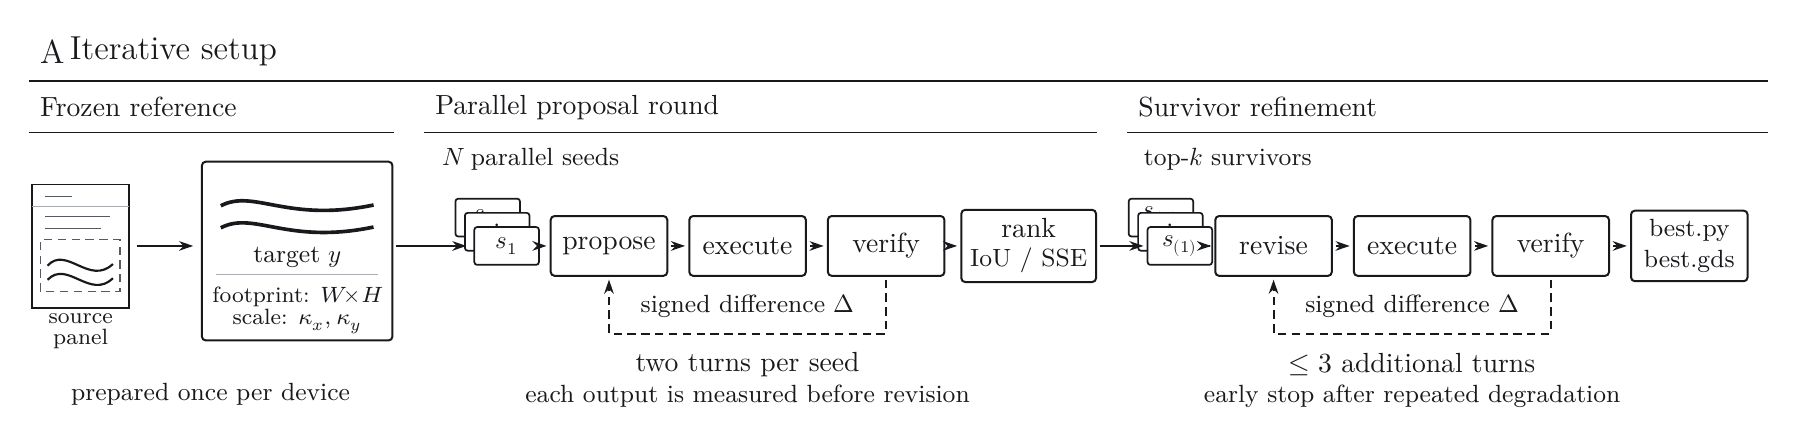
\begin{tikzpicture}[
  x=1cm,
  y=1cm,
  every node/.style={font=\normalsize, text=ink},
  panelletter/.style={font=\large},
  paneltitle/.style={font=\large, anchor=west},
  stageheading/.style={font=\normalsize, anchor=west},
  process/.style={
    draw=ink,
    line width=0.72pt,
    rounded corners=1.4pt,
    fill=white,
    minimum width=1.48cm,
    minimum height=0.76cm,
    inner sep=3.2pt,
    align=center
  },
  model/.style={process},
  verifier/.style={process},
  stack/.style={
    draw=ink,
    line width=0.62pt,
    rounded corners=1pt,
    fill=white,
    minimum width=0.82cm,
    minimum height=0.48cm,
    inner sep=2pt,
    align=center,
    font=\small
  },
  flow/.style={
    -{Stealth[length=1.80mm,width=1.22mm]},
    draw=ink,
    line width=0.74pt,
    shorten <=1.15pt,
    shorten >=1.15pt
  },
  dataflow/.style={
    -{Stealth[length=1.80mm,width=1.22mm]},
    draw=ink,
    line width=0.74pt,
    shorten <=1.15pt,
    shorten >=1.15pt
  },
  selectedflow/.style={
    -{Stealth[length=1.80mm,width=1.22mm]},
    draw=ink,
    line width=0.74pt,
    shorten <=1.15pt,
    shorten >=1.15pt
  },
  feedback/.style={
    -{Stealth[length=1.80mm,width=1.22mm]},
    draw=ink,
    line width=0.74pt,
    densely dashed,
    shorten <=1.0pt,
    shorten >=1.0pt
  },
  note/.style={font=\small, text=ink, align=center},
  smalllabel/.style={font=\small, align=center},
]

\node[panelletter, anchor=west] at (0.20,5.65) {A};
\node[paneltitle] at (0.58,5.65) {Iterative setup};
\draw[ink, line width=0.72pt] (0.18,5.27) -- (22.27,5.27);

\node[stageheading] at (0.20,4.94) {Frozen reference};
\draw[ink, line width=0.58pt] (0.18,4.62) -- (4.82,4.62);

\node[stageheading] at (5.22,4.94) {Parallel proposal round};
\draw[ink, line width=0.58pt] (5.20,4.62) -- (13.75,4.62);

\node[stageheading] at (14.15,4.94) {Survivor refinement};
\draw[ink, line width=0.58pt] (14.13,4.62) -- (22.27,4.62);

% ---------------------------------------------------------------------------
% Stage 1 -- prepare the immutable target and physical calibration once.
% Source-paper panel icon.
\draw[ink, line width=0.62pt, fill=white]
  (0.22,2.39) rectangle (1.45,3.96);
\draw[rulegray, line width=0.46pt]
  (0.22,3.68) -- (1.45,3.68);
\draw[inksoft, line width=0.45pt]
  (0.39,3.81) -- (0.73,3.81)
  (0.39,3.55) -- (1.21,3.55)
  (0.39,3.40) -- (1.10,3.40);
\draw[ink, line width=0.78pt]
  (0.42,2.93) .. controls (0.66,3.19) and (0.95,2.67) .. (1.25,2.95);
\draw[ink, line width=0.78pt]
  (0.42,2.75) .. controls (0.67,3.01) and (0.96,2.49) .. (1.25,2.77);
\draw[inksoft, line width=0.48pt, densely dashed]
  (0.33,2.60) rectangle (1.34,3.26);
\node[font=\footnotesize, align=center] at (0.84,2.10)
  {source\\[-2pt]panel};

% Preparation arrow; standardization and calibration are stated in the caption.
\draw[dataflow] (1.52,3.18) -- (2.31,3.18);

% Frozen benchmark bundle.
\draw[ink, line width=0.72pt, rounded corners=1.4pt, fill=white]
  (2.38,1.98) rectangle (4.80,4.25);
\draw[ink, line width=1.32pt]
  (2.62,3.69) .. controls (3.04,3.91) and (3.46,3.47) .. (4.56,3.70);
\draw[ink, line width=1.32pt]
  (2.62,3.41) .. controls (3.04,3.63) and (3.46,3.19) .. (4.56,3.42);
\node[smalllabel] at (3.59,3.03) {target $y$};
\draw[rulegray, line width=0.42pt] (2.56,2.82) -- (4.62,2.82);
\node[font=\footnotesize] at (3.59,2.53)
  {footprint: $W{\times}H$};
\node[font=\footnotesize] at (3.59,2.22)
  {scale: $\kappa_x,\kappa_y$};
\node[note] at (2.49,1.29) {prepared once per device};

% The same frozen reference is supplied to every independent seed.
\draw[dataflow] (4.80,3.18) -- (5.78,3.18);

% ---------------------------------------------------------------------------
% Stage 2 -- N independent seeds, each receiving two measured revision turns.
\node[smalllabel, anchor=west] at (5.31,4.28) {$N$ parallel seeds};
\node[stack] (seedback) at (6.01,3.54) {$s_N$};
\node[stack] (seedmid)  at (6.13,3.36) {$\vdots$};
\node[stack] (seedfront) at (6.25,3.18) {$s_1$};

\node[model]    (propose1) at (7.55,3.18) {propose};
\node[process]  (execute1) at (9.31,3.18) {execute};
\node[verifier] (verify1)  at (11.07,3.18) {verify};
\node[verifier, minimum width=1.58cm] (rank) at (12.88,3.18)
  {rank\\[-1.5pt]{\small IoU / SSE}};

\draw[flow] (seedfront.east) -- (propose1.west);
\draw[flow] (propose1.east) -- (execute1.west);
\draw[flow] (execute1.east) -- (verify1.west);
\draw[selectedflow] (verify1.east) -- (rank.west);

\draw[feedback]
  (verify1.south) -- ++(0,-0.72) -| (propose1.south);
\node[smalllabel, fill=white, inner xsep=3pt]
  at (9.31,2.42) {signed difference $\Delta$};
\node[font=\normalsize] at (9.31,1.67) {two turns per seed};
\node[note] at (9.31,1.27)
  {each output is measured before revision};

% ---------------------------------------------------------------------------
% Stage 3 -- only survivors receive up to three additional diff-guided turns.
\node[smalllabel, anchor=west] at (14.22,4.28) {top-$k$ survivors};
\node[stack] (survback) at (14.56,3.54) {$s_{(k)}$};
\node[stack] (survmid)  at (14.68,3.36) {$\vdots$};
\node[stack] (survfront) at (14.80,3.18) {$s_{(1)}$};

% Rank all seed candidates, then retain the high-scoring subset.
\draw[selectedflow] (rank.east) -- (survfront.west);

\node[model] (revise) at (15.99,3.18) {revise};
\node[process] (execute2) at (17.75,3.18) {execute};
\node[verifier] (verify2) at (19.51,3.18) {verify};
\node[process, font=\small] (best) at (21.27,3.18)
  {best.py\\best.gds};

\draw[flow] (survfront.east) -- (revise.west);
\draw[flow] (revise.east) -- (execute2.west);
\draw[flow] (execute2.east) -- (verify2.west);
\draw[selectedflow] (verify2.east) -- (best.west);

\draw[feedback]
  (verify2.south) -- ++(0,-0.72) -| (revise.south);
\node[smalllabel, fill=white, inner xsep=3pt]
  at (17.75,2.42) {signed difference $\Delta$};
\node[font=\normalsize] at (17.75,1.67)
  {$\leq 3$ additional turns};
\node[note] at (17.75,1.27)
  {early stop after repeated degradation};

\end{tikzpicture}
\end{document}
